% Slide aspect ratio, theme and color theme
\documentclass[aspectratio=169]{beamer}
\usetheme{metropolis}
\usecolortheme[snowy]{owl}

% Modern font setup
\usepackage{fontspec}
\usepackage{unicode-math}

% Font selection
\setmainfont{Fira Sans}
\setsansfont{Fira Sans}
\setmonofont[
  UprightFont   = *,
  BoldFont      = *-Bold,
  ItalicFont    = *,    % <-- force regular to be used as “italic”
  BoldItalicFont= *-Bold        % <-- or omit if you don’t need Bold Italic
]{Fira Code}
% \setmathfont{Fira Math}

% Language and layout
\usepackage[utf8]{inputenc}
\usepackage[brazil]{babel}

% Good to keep
\usepackage{amsmath}
\usepackage{graphicx}
\usepackage{url}
\usepackage{xcolor}
\usepackage{xstring}
\usepackage{outlines}

% Bibliography
\usepackage[backend=biber,style=authoryear]{biblatex}
\addbibresource{references.bib}
\renewcommand*{\nameyeardelim}{\addcomma\space}
\renewcommand*{\bibfont}{\color{black}\small}
\setbeamercolor{bibliography item}{fg=black}
\setbeamercolor{bibliography entry author}{fg=black}
\setbeamercolor{bibliography entry title}{fg=black}
\setbeamercolor{bibliography entry location}{fg=black}
\setbeamercolor{bibliography entry note}{fg=black}

% Wrapper for figures
\newcommand{\insertfigure}[3]{
  \StrBehind{#1}{/}[\FileWithExt]
  \StrBefore{\FileWithExt}{.}[\FileName]
  \begin{figure}[h!]
    \vspace{0.25cm}
    \centering
    \includegraphics[width=#3\linewidth]{#1}
    \caption{#2}
    \label{fig:\FileName}
  \end{figure}
}

% Shortcuts for MDP variables
\newcommand{\St}{\mathbf{S}}
\newcommand{\A}{\mathbf{A}}
\newcommand{\R}{\mathbf{R}}
\newcommand{\Ptr}{\mathbf{P}}
\newcommand{\Obs}{\mathbf{O}}

% END PREAMBLE

\title{Sintetizando episódios de treino via abstração de jogos em Aprendizado por Reforço}
\author{Marcelo Augusto Salomão Ganem}
\institute{Departamento de Ciência da Computação \\ Universidade Federal de Minas Gerais}
\date{\today}
\begin{document}

\makeatletter

\begin{frame}
\titlepage
\end{frame}

\begin{frame}{Resumo}
    \begin{outline}
        \1 Sintetizar episódios de treino em aprendizado por reforço a partir de abstrações de jogos baseadas na sintaxe Machinations, traduzindo-as formalmente em MDPs. \\
        \1 Definimos nós, gatilhos, conexões de recursos e modificadores como componentes de um diagrama cuja ativação e transferência de recursos geram a dinâmica de transição de estados observáveis e parcialmente observáveis.
    \end{outline}
\end{frame}

\begin{frame}{Resumo}
    \begin{outline}
        \1 Modelamos dois jogos clássicos — Blackjack e Monopoly — sob essa representação simplificada.
        \1 Buscamos aprender a política ótima no ambiente simulado de Monopoly: Deep Q-Networks (DQNs) não convergiram, enquanto agentes treinados com Proximal Policy Optimization (PPO) superaram a linha de base aleatória porém ainda apresentaram desempenho limitado em razão da alta estocasticidade e recompensas esparsas.
    \end{outline}
\end{frame}
% \begin{frame}{Outline}
% \tableofcontents
% \end{frame}


\section{Contexto}

\begin{frame}{Modelagens representativas}
    \begin{outline}
        \1 Como incluir conhecimento especializado em processos de treinamento que precisam generalizar para ambientes complexos?
        \1 \citeauthor{rl} (\citeyear{rl}) afirmam que, de certa forma, qualquer estratégia de construção de \textit{features} equivale a introduzir planejamento no cenário de aprendizado.
    \end{outline}
\end{frame}

\begin{frame}{Representando jogos}
    \begin{outline}
        \1 Enquanto alguns jogos apresentam espaços de estados limitados e claramente definidos (como o Blackjack), outros jogos como Go apresentam na ordem de $10^{170}$ estados legais possíveis\footnote{\url{https://tromp.github.io/go/legal.html}}.
        \1 Uma solução para isso é representar o espaço como um sinal bruto a partir do qual pode-se inferir uma função de valor extremamente não-linear com soluções de aprendizado profundo como DQNs \parencite{dqn}.
    \end{outline}
\end{frame}

\begin{frame}{Representando jogos}
    \begin{outline}
        \1 Uma alternativa antiga que reaparece na recorrentemente na literatura é a utilização de representações relacionais estruturadas de diversas maneiras no aprendizado \parencite{rrl}.
        \1 Nessa direção, diversos estudos exploram representações unificadas consistentes capazes de representar ambientes complexos -- especialmente no contexto de jogos.
    \end{outline}
\end{frame}

\begin{frame}{Diagramas \textit{Machinations}}
        \begin{columns}
            \begin{column}{0.5\textwidth}
                \vspace{0.25cm}

                A sintaxe Machinations introduz regras para a representação de jogos a uma variedade de níveis de abstração.
                \vspace{0.25cm}

                O modelo representa um jogo como um diagrama de nós e conexões de diversos tipos entre eles. Assim, o estado do jogo é a distribuição de \textbf{recursos} entre os nós.
            \end{column}
            \begin{column}{0.5\textwidth}
                \insertfigure
                    {figures/catan.png}
                    {Uma representação do jogo \textit{Settlers of Catan} sob a sintaxe de Machinations \parencite{machinations}}
                    {0.8}
            \end{column}
        \end{columns}
    
\end{frame}

\begin{frame}{Diagramas \textit{Machinations}}
    \begin{figure}[h!]
        \begin{columns}
            \begin{column}{0.6\textwidth}
                \vspace{0.5cm}
                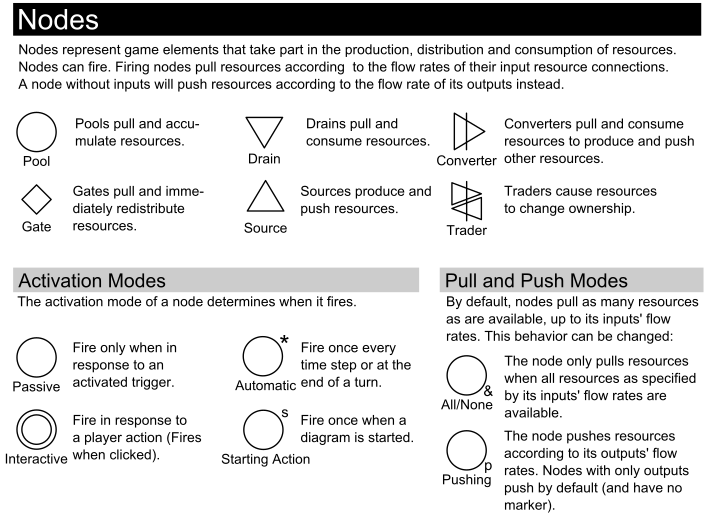
\includegraphics[width=1.0\linewidth]{figures/nodes.png}
            \end{column}
            \begin{column}{0.4\textwidth}
                \caption{Trecho do Apêndice A de \textit{Engineering Emergence} \parencite{machinations} descrevendo elementos básicos dos diagramas}
            \end{column}
        \end{columns}
        \label{fig:nodes}
    \end{figure}
\end{frame}

\begin{frame}{Diagramas \textit{Machinations}}
    \begin{columns}
        \begin{column}{0.5\textwidth}
	    A proposta da sintaxe é capturar e evidenciar relações na "economia interna" \ \parencite{machinations} do jogo a partir de suas regras. 
            \vspace{0.3cm}

    As regras definidas por \citeauthor{machinations} não são formais o suficiente para permitir implementação direta. Assim, parte desse trabalho é transcrever a definição descritiva para uma definição formal.
	    % A partir da definição dos elementos que compõem um diagrama e das conexões entre eles, é possível representar um único jogo de múltiplas maneiras.
        \end{column}
        \begin{column}{0.5\textwidth}
            \insertfigure
              {figures/monopoly.png}
              {\textit{Monopoly} (\citeyear{monopoly}) representado como um diagrama \textit{Machinations} \parencite{machinations}.}
              {1.0}
        \end{column}
    \end{columns}
\end{frame}

\section{Objetivos}

\begin{frame}{Objetivos}
    Utilizando diagramas Machinations como base, pretende-se \textbf{acelerar o treino de agentes de aprendizado por reforço via episódios sintetizados} como objetivo geral. Entendendo os diagramas como abstrações de problemas de aprendizado por reforço, o trabalho endereça especificamente as seguintes perguntas de pesquisa:
    \begin{outline}
        \1 Podemos utilizar as representações simplificadas no treino de agentes de aprendizado por reforço como uma pré-otimização com respeito à verdadeira política ótima?
        \1 É possível extrair informações úteis sobre jogos modelados na sintaxe proposta a partir do comportamento de agentes de aprendizado por reforço?
    \end{outline}
\end{frame}

\section{Trabalhos Relacionados}
\begin{frame}{Curriculum Learning}
    O trabalho de \citeauthor{curriculum-learning} (\citeyear{curriculum-learning}) fundamenta a ideia de aprendizado por tarefas sucessivas de complexidade crescente. Especificamente, dada a coerência entre os ambientes e tarefas apresentadas, \citeauthor{curriculum-learning} provam que essa técnica \textbf{acelera a convergência} no treino.

    A princípio, entendemos o aprendizado no ambiente modelado em Machinations como a tarefa inicial (de otimização mais genérica), e o aprendizado no ambiente completo como a segunda e última tarefa do currículo (refinando a otimização anterior).
\end{frame}
\begin{frame}{A modeling environment for reinforcement learning in games}
    \citeauthor{modeling-rl-games} \citeyear{modeling-rl-games} declaram um objetivo muito semelhante para o ambiente AI4U\footnote{\url{https://github.com/gilzamir18/AI4U}}.
    \vspace{0.3cm}

\begin{quote}
    [...] to enable the reproducibility of methods and results; \textbf{to simplify the way of designing reinforcement learning algorithms in games;} and to enhance the readability of RL agents.
\end{quote}

% A solução apresentada pelos autores se centraliza na definição de uma ontologia de elementos e comportamentos compatíveis com definições comuns em engines de jogos, tal que desenvolvedores são capazes de especificar elementos das interações e regras desejadas para reforçar comportamentos em personagens não jogáveis. Observamos, assim, uma evidência da eficácia da introdução de uma simplificação relacional estruturada como linguagem única para a produção de uma solução em aprendizado por reforço.

\end{frame}


\section{Metodologia}

\begin{frame}{Metodologia}
    \begin{outline}[enumerate]
	\1 Definição de diagramas Machinations como MDPs
	\1 Implementação do MDP e ambientes de aprendizado para:
            \2 Blackjack
            \2 Monopoly
	\1 Realizar o treino de agentes de RL no MDP abstrativo
    \1 Verificar a capacidade de convergência dos agentes nas simulações construídas\footnote{Especificamente, analisamos as soluções de DQN e PPO para o jogo Monopoly}.
    \1 Verificar o que a relação entre os ambientes modelados e as políticas aprendidas revelam sobre a aplicabilidade dos diagramas propostos.
    \1 MSI II: verificar a capacidade de transferência para simulações completas.
    \end{outline}
\end{frame}

\begin{frame}{Formalizando diagramas \textit{Machinations}}
    \begin{outline}
      \1 Definição
            \2 Diagrama $(V, E)$: nós e conexões com tipos, propriedades e estados\footnote{Não é um grafo simples: arestas para arestas $e:(v\rightarrow e')$.}.
      \1 Nós ($v\in V$)
         \2 Estado $X_{v,r,t}\in\mathbb{R}$: quantidade de recurso $r$ no tempo $t$.
         \2 Modos de ativação: passivo (por gatilhos); automático (a todo instante); interativo (ação do agente); não-determinístico (amostra aleatória).
         \2 Distribuição inicial opcional: reamostra ao ativar.
      \1 Conexões e Predicados
         \2 Predicado $P_e$: condição matemática em função do nó de origem.
         \2 Gatilhos ($E^G$): passivos vs.\ automáticos, possuem um predicado $P_e$.
         \2 Ativadores ($E^A$): impõem $P_e$ para ativar ou bloquear nós/conexões.
  \end{outline}
\end{frame}

\begin{frame}{Formalizando diagramas \textit{Machinations}}
    \begin{outline}
      \1 Transferência de Recursos ($E^R$)
         \2 Cada ativação envia $T_{e,t}$ unidades de $\tau_e$ do nó origem ao destino.
         \2 Respeita mesmas regras de predicados e ativadores dos nós.
      \1 Modificadores ($E^M$)
         \2 Alvo pode ser nó ou conexão de recurso.
         \2 A cada instante, adiciona:
            \3 $\dot{T}_e \times X_{v,\tau_{\text{SRC}},t}$ ao estado do alvo.
         \2 Taxa $\dot{T}_e$ é fixa (não depende de $t$).
      \1 Resumo da Dinâmica
         \2 Ativação de nó $\Rightarrow$ dispara gatilhos + conexões.
         \2 Modificadores geram padrões assintóticos de fluxo.
  \end{outline}
\end{frame}

\begin{frame}
\begin{figure}[h!]
    \centering
    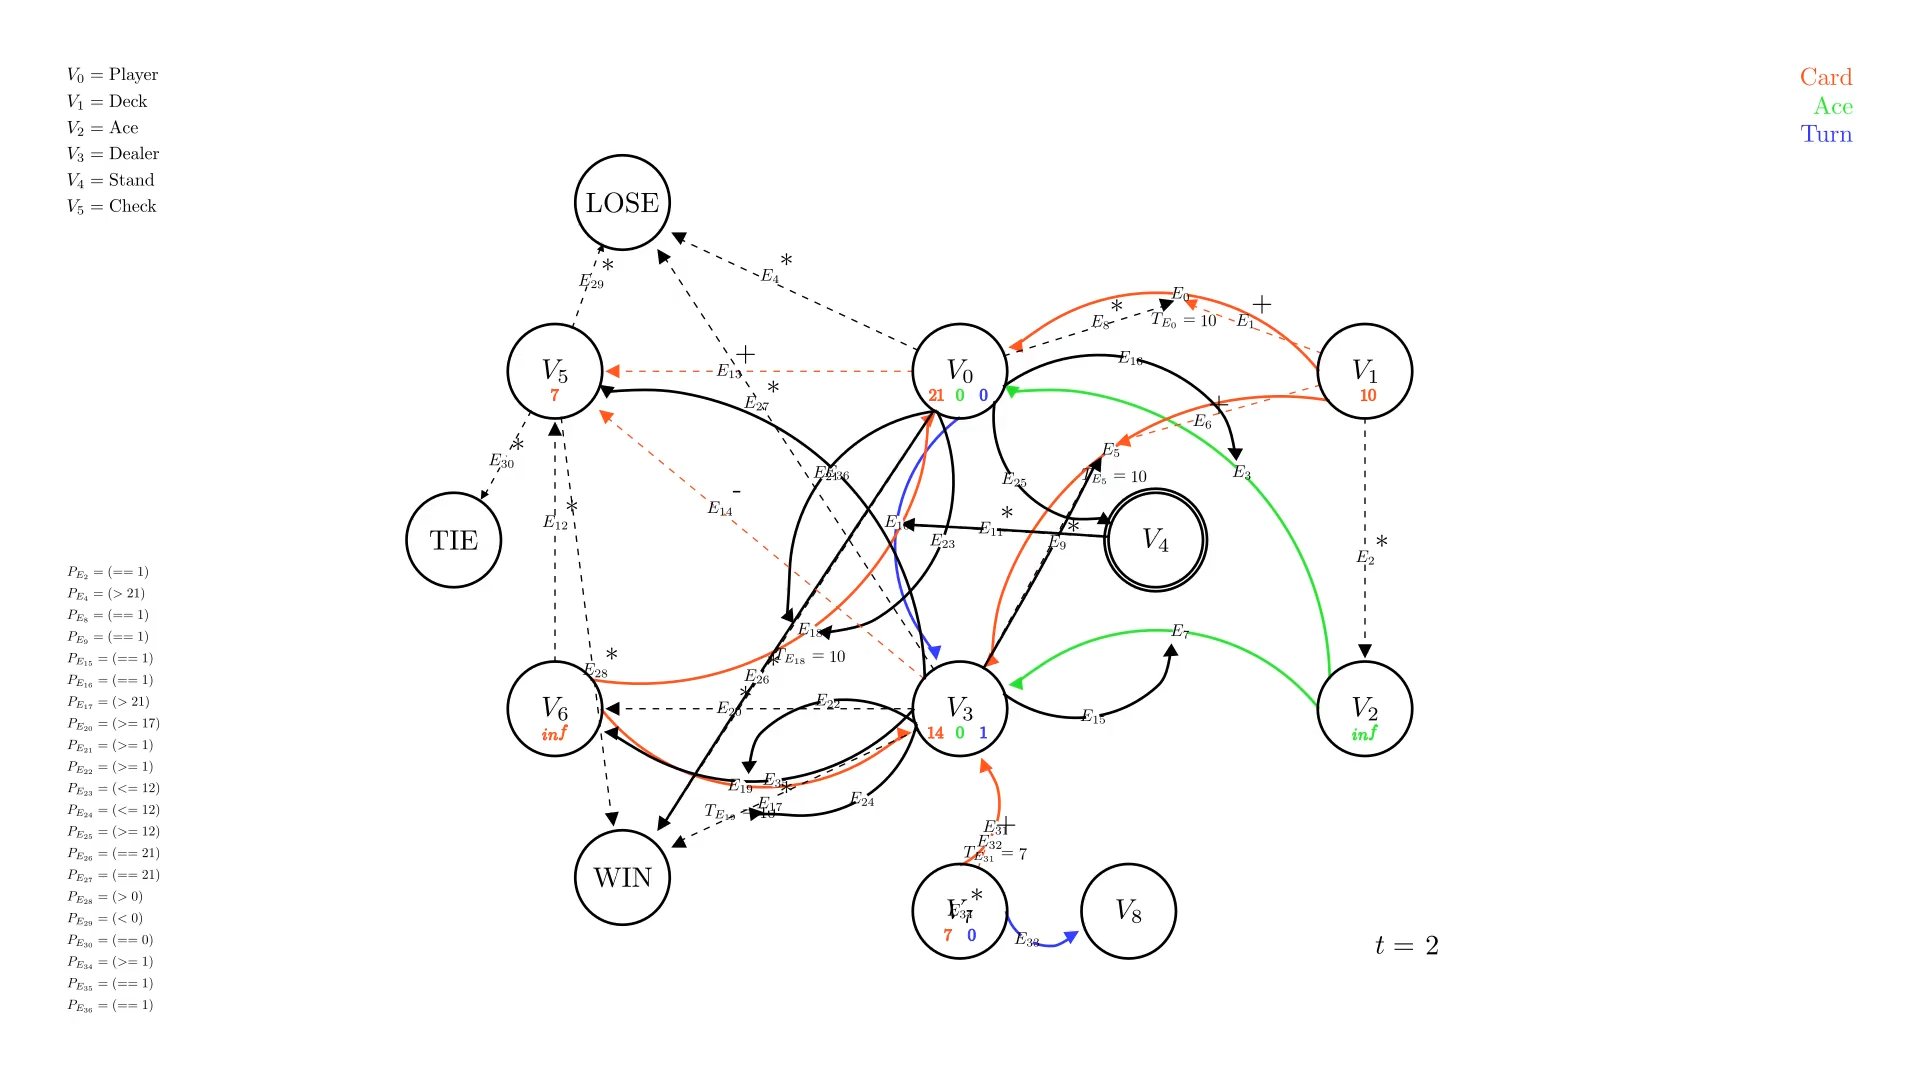
\includegraphics[width=0.9\linewidth]{figures/Blackjack.png}
    \caption{Representação do jogo \textit{Blackjack} sob a sintaxe implementada.}
    \label{fig:blackjack}
\end{figure}
\end{frame}

\begin{frame}
\begin{figure}[h!]
    \centering
    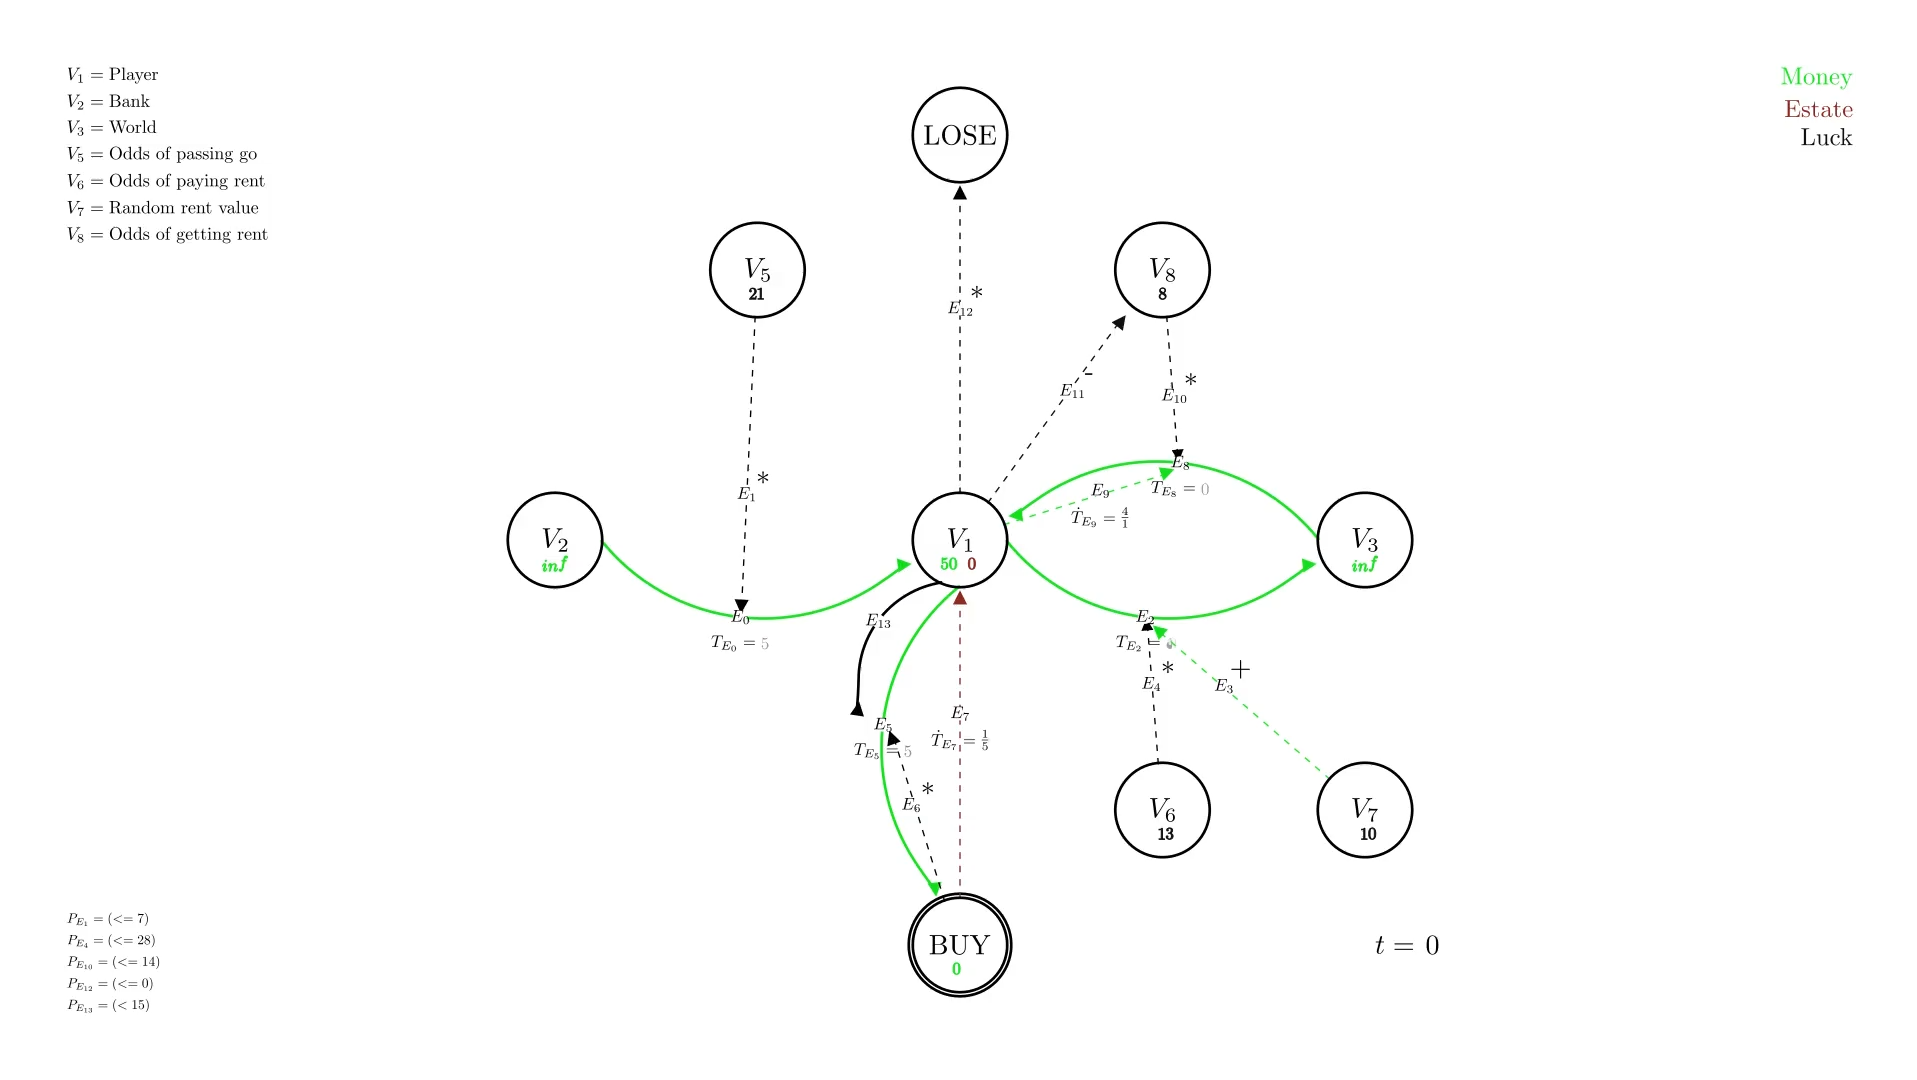
\includegraphics[width=0.9\linewidth]{figures/Monopoly.png}
    \caption{Representação do jogo \textit{Monopoly} sob a sintaxe implementada.}
    \label{fig:my-monopoly}
\end{figure}
\end{frame}

\begin{frame}{Definindo o POMDP}
    \begin{columns}
	\begin{column}{0.5\textwidth}
        Definimos subconjuntos $X^O$ e $T^O$ correspondentes aos nós e conexões de recursos observáveis tal que um estado $S_t \in \mathbf{S}$ tem a forma:

        $$
        S_t = \{X^O_t, T^O_t\}
        $$

	    Ações são definidas como o conjunto potência dos vértices interativos: 
        $$
        \A = \mathcal{P}(\{ v \in V^A \})
        $$
	\end{column}
	\begin{column}{0.5\textwidth}
        Definimos pesos $\omega$ e $\rho$ para cada nó e conexão de recursos, respectivamente. Seguindo o princípio de \textit{potential-based shaping} \parencite{potential-rl}, temos:
        $$
        \Phi(s) = \sum_{v\in V^{\Phi}}\sum_{r \in R^{\Phi}}\omega_{v,r}\,x_{v,r}+\sum_{e\in E^{R^{\Phi}}}\rho_{e}\,T_{e}
        $$
        $$
        \R(s,a,s') = \Phi(s') \;-\; \Phi(s)
        $$
    \end{column}
    \end{columns}
\end{frame}

\begin{frame}{Aprendizado}
    \begin{outline}
	\1 Objetivo: sobreviver até $t = 30$ na simulação de Monopoly.
	    \2 Baselines: agente que nunca compra, agente que compra 50\% do tempo.
    \1 Recompensas avaliadas ao final:\footnote{Recompensas intermediárias foram omitidas para evitar induzir explicitamente o comportamento do agente, dada a simplicidade do problema.}
        \2 $1 + R(s)$ para vitória, $-1 + \min(0, R(s))$ para derrota.
	\vspace{0.25cm}
        \1 Aprendizado profundo: DQNs (falham), PPO (supera as baselines)
	    \2 Responder a padrões no diagrama % Caso do monopoly
	    \2 Lidar com espaços de estado maiores % Muitos nós, tipos de recurso e conexões
    \end{outline}
\end{frame}

\begin{frame}

    \begin{table}[h!]
        \caption{Hiperparâmetros utilizados na aplicação de PPO ao ambiente que simula o jogo Monopoly}
        \begin{center}
            \begin{tabular}{|l|c|}
                \hline
                \textbf{Hiperparâmetro}              & \textbf{Valor}    \\
                \hline
                Taxa de aprendizado                  & $5\times10^{-4}$  \\
                \hline
                Fator de desconto                    & $0.98$            \\
                \hline
                Suavização GAE                       & $0.95$            \\
                \hline
                Comprimento do rollout               & $4096$            \\
                \hline
                Tamanho do batch                     & $128$             \\
                \hline
                Épocas por atualização               & $15$              \\
                \hline
                Intervalo de clipping                & $0.3$             \\
                \hline
                Coeficiente de entropia              & $0.05$            \\
                \hline
                Coeficiente de perda de valor        & $0.5$             \\
                \hline
                Norma máxima do gradiente            & $1.0$             \\
                \hline
            \end{tabular}
        \label{tab:ppo_hyperparams}
        \end{center}
    \end{table}

\end{frame}


\begin{frame}{Resultados}
                \begin{figure}[htpb]
                    \centering
                    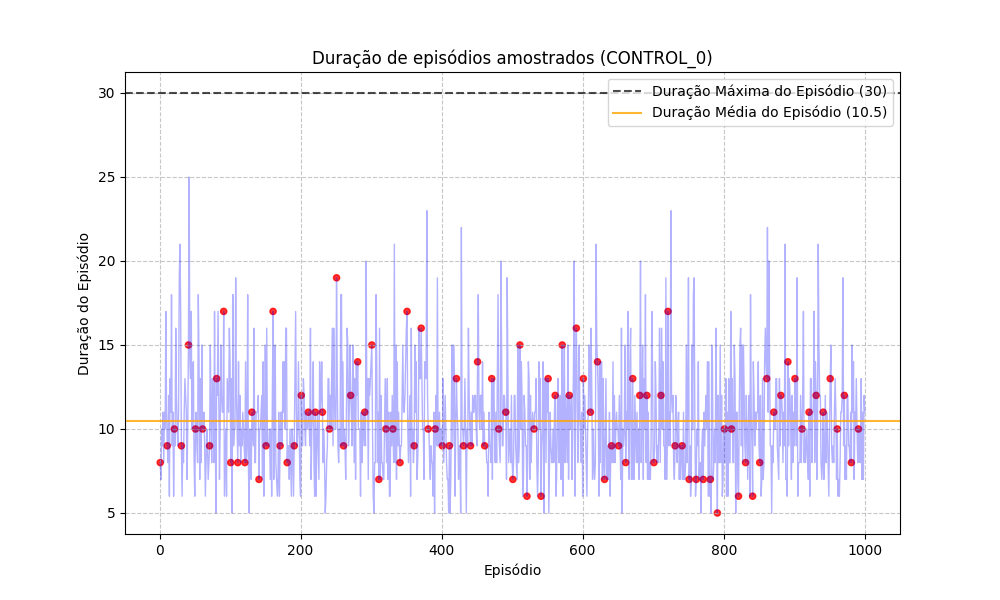
\includegraphics[width=0.85\linewidth]{figures/episode_lengths_control_0.png}
                    %\caption{Duração do episódio para 1000 episódios executados com um agente que nunca compra propriedades.}
                    \label{fig:ep_lens_control_0}
                \end{figure}
\end{frame}
\begin{frame}{Resultados}
                \begin{figure}[htpb]
                    \centering
                    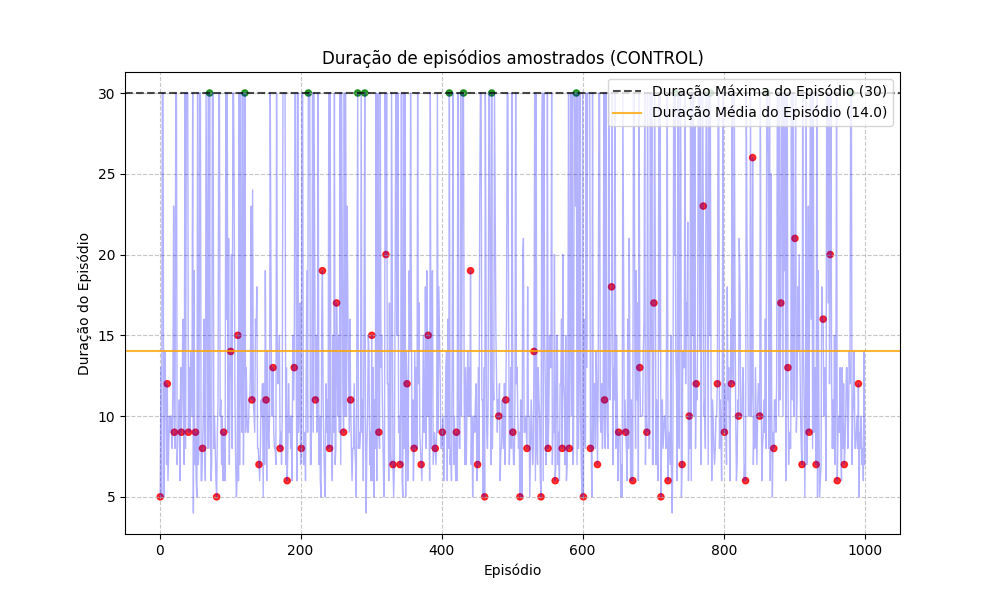
\includegraphics[width=0.85\linewidth]{figures/episode_lengths_control.png}
                    %\caption{Duração do episódio para 1000 episódios executados com um agente de escolha aleatória.}
                    \label{fig:ep_lens_control}
                \end{figure}
\end{frame}

\begin{frame}{Resultados}
        \begin{figure}[htpb]
            \centering
            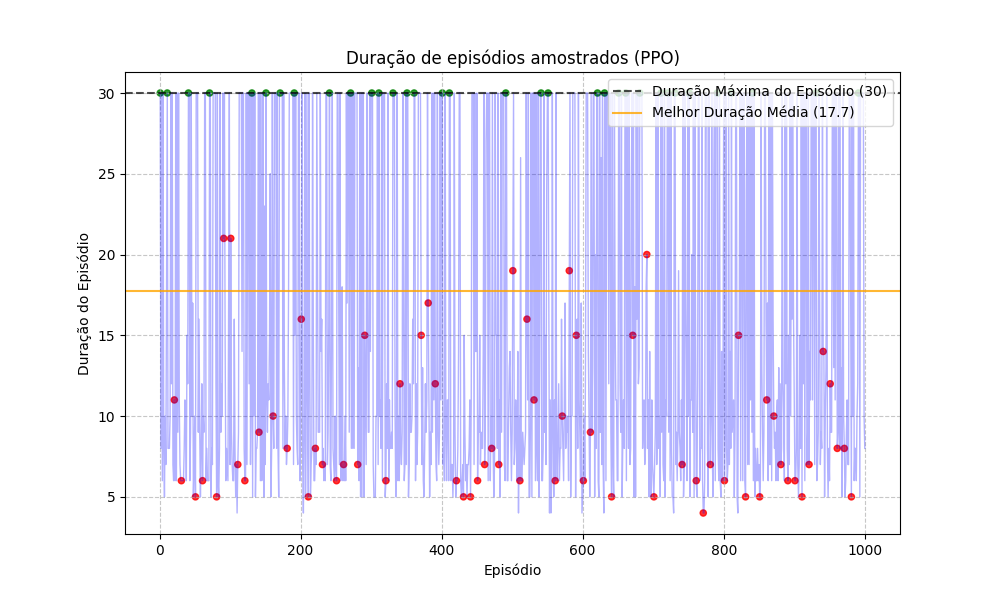
\includegraphics[width=0.85\linewidth]{figures/episode_lengths_ppo.png}
            %\caption{Duração do episódio para 1000 episódios executados com um agente treinado por PPO durante 200.000 episódios.}
            \label{fig:ep_lens_ppo}
        \end{figure}
\end{frame}
\begin{frame}{Resultados}
        \begin{figure}[htpb]
            \centering
            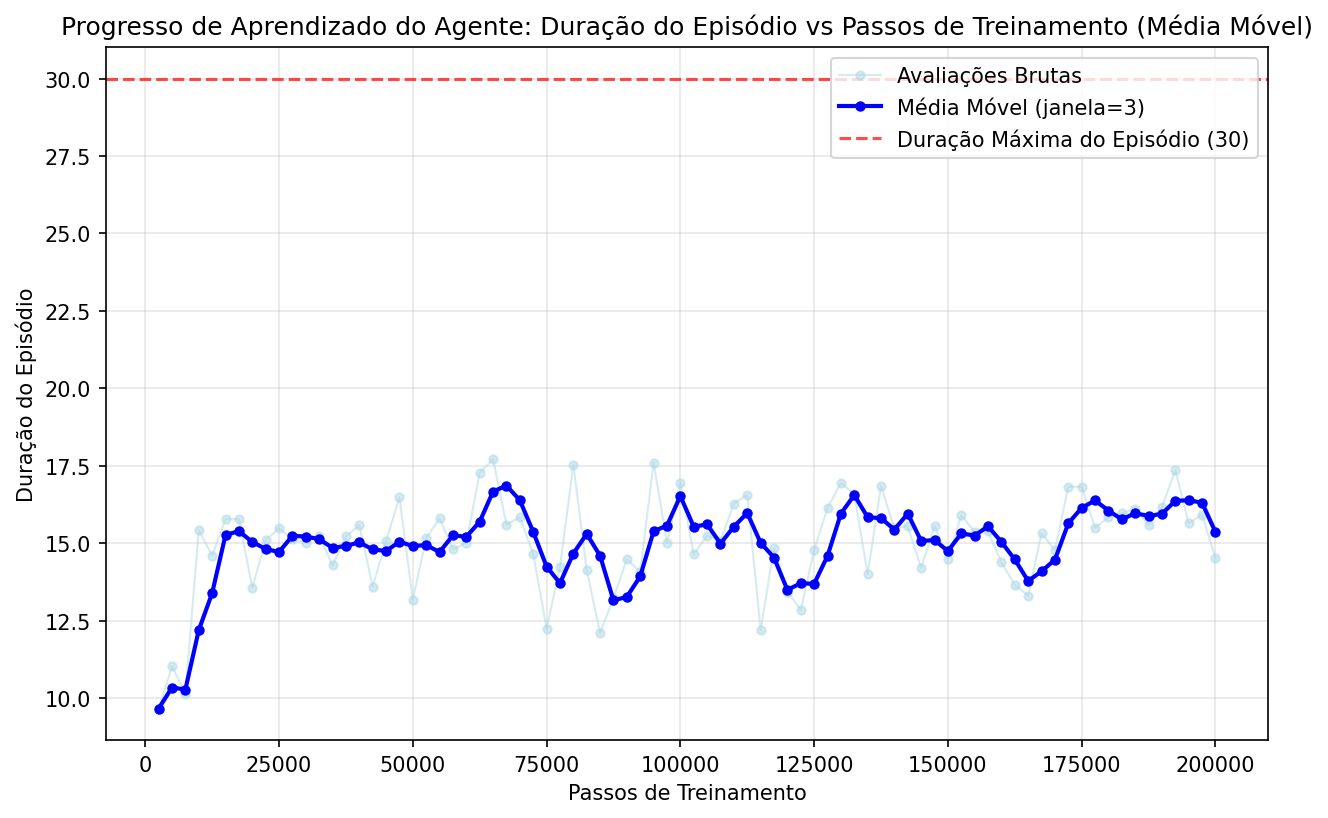
\includegraphics[width=0.85\linewidth]{figures/eval_progress.png}
            %\caption{Progresso do treinamento do agente, medido pelo tempo de sobrevivência médio ao longo de 100 episódios de avaliação, executados a cada 2.500 etapas do treinmanto.}
            \label{fig:eval_progress}
        \end{figure}
\end{frame}

\begin{frame}{Considerações}
  \begin{outline}
  \1 \textbf{Qualidade das Modelagens}
     \2 Concessões: sintaxe implementada ≠ sintaxe de Engineering Emergence
      \2 Caso comum em implementações acadêmicas (descrições mais livres)\footnote{\url{https://machinations.io/resources/academic-research-publications}}
  \1 \textbf{Estocasticidade dos Ambientes}
     \2 Abstração lógica/probabilística oculta mecânicas completas (ex.: Monopoly)
     \2 Sinal de recompensa mais ruidoso → dificuldade em capturar relações sutis
  \end{outline}
\end{frame}

\begin{frame}{Trabalhos Futuros}
  \begin{outline}
  \1 \textbf{Transferência via Curriculum Learning}
     \2 Hípótese: diagramas progressivamente complexos melhoram a generalização  
     \2 Investigação necessária sobre sequência ótima de complexidade  
  \1 \textbf{Abordagens Model-Based}
     \2 Aplicar Monte Carlo com aproximação de funções em problemas curtos e estocásticos  
     \2 “Exploring starts” direcionado: usar modelagem para começar com uma melhor função de transição 
  \end{outline}
\end{frame}

\begin{frame}[shrink=5]
    \vspace{0.75cm}
    \printbibliography
\end{frame}


\end{document}

